\begin{frame}{Diagrama de Tempo (\textit{Waveform})}
	\par Quando fazemos o diagrama de tempo ou o \textit{waveform} apresentamos ao circuito uma sequência de  sinais de forma que o circuito responde a essa sequência gerando outras sequências. 
	\begin{itemize}
		\item Mostra os estados do circuito ao longo do tempo.
		\item Permite a visualização do comportamento do circuito durante o tempo.
	\end{itemize}
	\begin{figure}
		\centering
		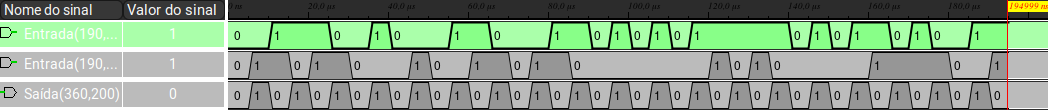
\includegraphics[width=\linewidth]{images/waveform01}
		\caption{Consegue saber qual porta é esta?}
		\label{fig:waveform01}
	\end{figure}
\end{frame}

\begin{frame}{Exercícios}
	\par Construção de Circuito a partir de Expressão Algébrica
	\begin{itemize}
		\item Dada a expressão algébrica \(F(x, y, z) = \overline{x} \cdot y + x \cdot \overline{y} \cdot z\), construa:
		\begin{enumerate}
			\item O circuito correspondente usando portas lógicas básicas (AND, OR, NOT).
			\item A tabela verdade que representa o comportamento da função.
			\item O diagrama de tempo (waveform) que mostra os estados do circuito para todas as combinações de \(x\), \(y\) e \(z\) ao longo do tempo.
		\end{enumerate}
	\end{itemize}
\end{frame}

\begin{frame}{Exercícios}
	\par Análise de Diagrama de Tempo
	\begin{figure}
		\centering
		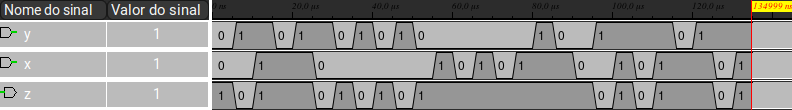
\includegraphics[width=0.7\linewidth]{images/waveform02}
		\label{fig:waveform02}
	\end{figure}
	\begin{columns}
		\column{.5\linewidth}
		\begin{itemize}
			\item Considerando o diagrama dado:
			\begin{enumerate}
				\item O circuito que pode gerar o comportamento mostrado no diagrama.
				\item A tabela verdade associada ao circuito.
				\item A expressão algébrica correspondente ao circuito.
			\end{enumerate}
		\end{itemize}
		\pause
		\column{.2\linewidth}
		\par Tabela verdade:
		\begin{center}
			\begin{tabular}{cc|c}
				$x$&$y$&$z$\\
				\hline
				$0$&$0$&$1$\\
				$0$&$1$&$0$\\
				$1$&$0$&$1$\\
				$1$&$1$&$1$\\
			\end{tabular}
		\end{center}		
		\par Expressão:
		$z =  \overline{y} +x$
		\column{.3\linewidth}
		\begin{figure}
			\centering
			% Important: If latex complains about unicode characters,
% please use "\usepackage[utf8x]{inputenc}" in your preamble
% You can change the size of the picture by putting it into the construct:
% 1) \resizebox{10cm}{!}{"below picture"} to scale horizontally to 10 cm
% 2) \resizebox{!}{15cm}{"below picture"} to scale vertically to 15 cm
% 3) \resizebox{10cm}{15cm}{"below picture"} a combination of above two
% It is not recomended to use the scale option of the tikzpicture environment.
\resizebox{4.5cm}{!}{
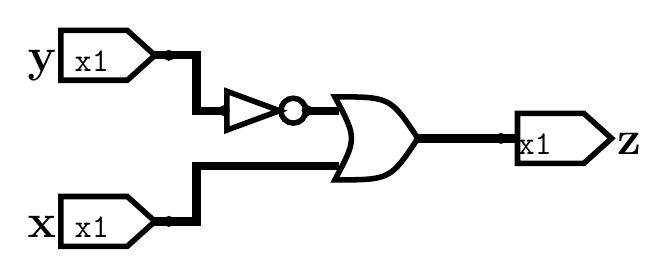
\begin{tikzpicture}[x=1pt,y=-1pt,line cap=rect]
\def\logisimfontA#1{\fontfamily{cmr}{#1}} % Replaced by logisim, original font was "SansSerif"
\def\logisimfontB#1{\fontfamily{cmtt}{#1}} % Replaced by logisim, original font was "Monospaced"
\definecolor{custcol_0_0_0}{RGB}{0, 0, 0}
\definecolor{custcol_ff_ff_ff}{RGB}{255, 255, 255}
\draw [line width=3.0pt, custcol_0_0_0 ]  (146.0,45.0) -- (176.0,45.0) ;
\draw [line width=3.0pt, custcol_0_0_0 ]  (106.0,35.0) -- (116.0,35.0) -- (116.0,35.0) ;
\draw [line width=2.0pt, custcol_0_0_0 ]  (146.0,45.0) .. controls  (136.0,30.0)  ..  (116.0,30.0) .. controls  (124.0,45.0)  ..  (116.0,60.0) .. controls  (136.0,60.0)  ..  (146.0,45.0) -- cycle ;
\draw [line width=2.0pt, custcol_0_0_0 ]  (96.0,35.0) -- (77.0,28.0) -- (77.0,42.0) -- cycle;
\draw [line width=2.0pt, custcol_0_0_0]  (101.0,35.0) ellipse (4.5 and 4.5 );
\fill [line width=2.0pt, custcol_0_0_0]  (106.0,35.0) ellipse (2.0 and 2.0 );
\fill [line width=2.0pt, custcol_0_0_0]  (76.0,35.0) ellipse (2.0 and 2.0 );
\draw [line width=3.0pt, custcol_0_0_0 ]  (180.0,45.0) -- (177.0,45.0) ;
\draw [line width=2.0pt, custcol_0_0_0 ]  (206.0,36.0) -- (216.0,45.0) -- (206.0,54.0) -- (182.0,54.0) -- (182.0,36.0) -- cycle;
\logisimfontB{\fontsize{12pt}{12pt}\selectfont\node[inner sep=0, outer sep=0, custcol_0_0_0, anchor=base west] at  (182.0,51.0)  {x1};}
\logisimfontA{\fontsize{16pt}{16pt}\fontseries{bx}\selectfont\node[inner sep=0, outer sep=0, custcol_0_0_0, anchor=base west] at  (218.0,51.0)  {z};}
\fill [line width=2.0pt, custcol_0_0_0]  (176.0,45.0) ellipse (2.0 and 2.0 );
\draw [line width=3.0pt, custcol_0_0_0 ]  (51.0,75.0) -- (56.0,75.0) -- (66.0,75.0) -- (66.0,55.0) -- (116.0,55.0) -- (116.0,55.0) ;
\draw [line width=2.0pt, custcol_0_0_0 ]  (41.0,84.0) -- (51.0,75.0) -- (41.0,66.0) -- (17.0,66.0) -- (17.0,84.0) -- cycle;
\logisimfontB{\fontsize{12pt}{12pt}\selectfont\node[inner sep=0, outer sep=0, custcol_0_0_0, anchor=base west] at  (22.0,81.0)  {x1};}
\logisimfontA{\fontsize{16pt}{16pt}\fontseries{bx}\selectfont\node[inner sep=0, outer sep=0, custcol_0_0_0, anchor=base west] at  (5.0,81.0)  {x};}
\fill [line width=2.0pt, custcol_0_0_0]  (56.0,75.0) ellipse (2.0 and 2.0 );
\draw [line width=3.0pt, custcol_0_0_0 ]  (51.0,15.0) -- (56.0,15.0) -- (66.0,15.0) -- (66.0,35.0) -- (76.0,35.0) ;
\draw [line width=2.0pt, custcol_0_0_0 ]  (41.0,24.0) -- (51.0,15.0) -- (41.0,6.0) -- (17.0,6.0) -- (17.0,24.0) -- cycle;
\logisimfontB{\fontsize{12pt}{12pt}\selectfont\node[inner sep=0, outer sep=0, custcol_0_0_0, anchor=base west] at  (22.0,21.0)  {x1};}
\logisimfontA{\fontsize{16pt}{16pt}\fontseries{bx}\selectfont\node[inner sep=0, outer sep=0, custcol_0_0_0, anchor=base west] at  (5.0,21.0)  {y};}
\fill [line width=2.0pt, custcol_0_0_0]  (56.0,15.0) ellipse (2.0 and 2.0 );
\end{tikzpicture}
}

			\label{fig:exe09}
		\end{figure}
	\end{columns}
\end{frame}


	\begin{frame}{Exemplo de min termos e max termos}
		\par Exemplo: Determinação de Função Lógica a partir de Tabela Verdade Usando Mintermos e Maxtermos
		
		\par{Tabela Verdade}
		
		\par Vamos considerar uma função booleana \(f(a, b, c)\) com três variáveis. Aqui está a tabela verdade:
		
		\[
		\begin{array}{|c|c|c|c|}
			\hline
			a & b & c & f(a, b, c) \\
			\hline
			0 & 0 & 0 & 0 \\
			0 & 0 & 1 & 1 \\
			0 & 1 & 0 & 0 \\
			0 & 1 & 1 & 1 \\
			1 & 0 & 0 & 1 \\
			1 & 0 & 1 & 1 \\
			1 & 1 & 0 & 0 \\
			1 & 1 & 1 & 0 \\
			\hline
		\end{array}
		\]
	\end{frame}
	
	\begin{frame}{Exemplo de min termos e max termos}
		\par{Determinação da Função Usando Mintermos}
		
		\textbf{Passo 1:} Identifique as linhas onde \(f(a, b, c) = 1\).
		
		\par As linhas onde a função vale 1 são:
		\begin{itemize}
			\item Linha 2: \(a = 0\), \(b = 0\), \(c = 1\)  \(\rightarrow\) Mintermo: \(a'b'c\)
			\item Linha 4: \(a = 0\), \(b = 1\), \(c = 1\)  \(\rightarrow\) Mintermo: \(a'bc\)
			\item Linha 5: \(a = 1\), \(b = 0\), \(c = 0\)  \(\rightarrow\) Mintermo: \(ab'c'\)
			\item Linha 6: \(a = 1\), \(b = 0\), \(c = 1\)  \(\rightarrow\) Mintermo: \(ab'c\)
		\end{itemize}
		
		\textbf{Passo 2:} Escreva a função como a soma (OR) desses mintermos.
		
		A função lógica pode ser expressa como a soma dos mintermos correspondentes:
		
		\[
		f(a, b, c) = a'b'c + a'bc + ab'c' + ab'c
		\]
	\end{frame}
	
	\begin{frame}{Exemplo de min termos e max termos}
		\par{Determinação da Função Usando Maxtermos}
		
		\textbf{Passo 1:} Identifique as linhas onde \(f(a, b, c) = 0\).
		
		As linhas onde a função vale 0 são:
		\begin{itemize}
			\item Linha 1: \(a = 0\), \(b = 0\), \(c = 0\)  \(\rightarrow\) Maxtermo: \((a + b + c)\)
			\item Linha 3: \(a = 0\), \(b = 1\), \(c = 0\)  \(\rightarrow\) Maxtermo: \((a + b' + c)\)
			\item Linha 7: \(a = 1\), \(b = 1\), \(c = 0\)  \(\rightarrow\) Maxtermo: \((a' + b + c)\)
			\item Linha 8: \(a = 1\), \(b = 1\), \(c = 1\)  \(\rightarrow\) Maxtermo: \((a' + b + c')\)
		\end{itemize}
		
		\textbf{Passo 2:} Escreva a função como o produto (AND) desses maxtermos.
		
		A função lógica pode ser expressa como o produto dos maxtermos correspondentes:
		
		\[
		f(a, b, c) = (a + b + c) \cdot (a + b' + c) \cdot (a' + b + c) \cdot (a' + b + c')
		\]
	\end{frame}
	
	\begin{frame}{Exemplo de min termos e max termos}
		\par{Resumo}
		
		\begin{itemize}
			\item \textbf{Usando Mintermos (Soma de Produtos Canônica):} A função é expressa como a soma (OR) dos mintermos das linhas onde a função vale 1.
			\item \textbf{Usando Maxtermos (Produto de Somas Canônica):} A função é expressa como o produto (AND) dos maxtermos das linhas onde a função vale 0.
		\end{itemize}
		
	\end{frame}


\begin{frame}{Definição e Propriedades}
	\begin{itemize}
		\item A implementação canônica de uma função booleana que seleciona os produtos das variáveis onde o resultado é 1.
		\item Propriedades:
		\begin{itemize}
			\item Unicidade: Existe uma única SOP canônica para cada função booleana.
			\item Importância: Útil na análise e síntese de circuitos digitais.
			\item Minimização: Pode ser simplificada com Mapas de Karnaugh ou Quine-McCluskey.
		\end{itemize}
	\end{itemize}
\end{frame}

\begin{frame}{Exemplo de SOP Canônica}
	\begin{itemize}
		\item Considere a função F(A, B, C) definida pela tabela verdade:
		\item \textbf{Tabela Verdade:}
		\begin{tabular}{|c|c|c|c|}
			\hline
			A & B & C & F(A, B, C) \\
			\hline
			0 & 0 & 0 & 0 \\
			0 & 0 & 1 & 1 \\
			0 & 1 & 0 & 0 \\
			0 & 1 & 1 & 1 \\
			1 & 0 & 0 & 1 \\
			1 & 0 & 1 & 1 \\
			1 & 1 & 0 & 0 \\
			1 & 1 & 1 & 1 \\
			\hline
		\end{tabular}
		\item \textbf{Mintermos:}
		\begin{itemize}
			\item A'B'C, A'BC, AB'C', ABC', ABC
		\end{itemize}
		\item \textbf{SOP Canônica:}
		\[
		F(A,B,C) = A'B'C + A'BC + AB'C' + ABC' + ABC
		\]
	\end{itemize}
\end{frame}

\section{Produto de Somas Canônica (POS)}

\begin{frame}{Definição e Propriedades}
	\begin{itemize}
		\item Forma canônica que seleciona as somas das variáveis onde o resultado é 0.
		\item Propriedades:
		\begin{itemize}
			\item Unicidade: Existe uma única POS canônica para cada função booleana.
			\item Importância: Utilizada em design digital para implementar lógica com portas OR e AND.
			\item Minimização: Pode ser simplificada como a SOP canônica.
		\end{itemize}
	\end{itemize}
\end{frame}

\begin{frame}{Exemplo de POS Canônica}
	\begin{itemize}
		\item \textbf{Tabela Verdade:}
		\begin{tabular}{|c|c|c|c|}
			\hline
			A & B & C & F(A, B, C) \\
			\hline
			0 & 0 & 0 & 0 \\
			0 & 0 & 1 & 1 \\
			0 & 1 & 0 & 0 \\
			0 & 1 & 1 & 1 \\
			1 & 0 & 0 & 1 \\
			1 & 0 & 1 & 1 \\
			1 & 1 & 0 & 0 \\
			1 & 1 & 1 & 1 \\
			\hline
		\end{tabular}
		\item \textbf{Maxtermos:}
		\begin{itemize}
			\item (A + B + C), (A + B' + C), (A' + B + C')
		\end{itemize}
		\item \textbf{POS Canônica:}
		\[
		F(A,B,C) = (A + B + C) \cdot (A + B' + C) \cdot (A' + B + C')
		\]
	\end{itemize}
\end{frame}

\section{Mintermos e Maxtermos}

\begin{frame}{Definição de Mintermos e Maxtermos}
	\begin{itemize}
		\item \textbf{Mintermo:}
		\begin{itemize}
			\item Produto de todas as variáveis complementadas ou não.
			\item Exemplo: `A'B'C`
		\end{itemize}
		\item \textbf{Maxtermo:}
		\begin{itemize}
			\item Soma de todas as variáveis complementadas ou não.
			\item Exemplo: `(A + B + C')`
		\end{itemize}
	\end{itemize}
\end{frame}

\begin{frame}{Exercícios}
	\par Criação de Circuito a partir da Tabela Verdade
	\begin{itemize}
		\item Dada a seguinte tabela verdade:
		\[
		\begin{array}{|c|c|c|c|}
			\hline
			x & y & z & F(x, y, z) \\
			\hline
			0 & 0 & 0 & 0 \\
			0 & 0 & 1 & 1 \\
			0 & 1 & 0 & 0 \\
			0 & 1 & 1 & 1 \\
			1 & 0 & 0 & 1 \\
			1 & 0 & 1 & 0 \\
			1 & 1 & 0 & 0 \\
			1 & 1 & 1 & 1 \\
			\hline
		\end{array}
		\]
		\begin{enumerate}
			\item Construa o circuito digital que implementa essa função.
			\item Derive a expressão algébrica na forma de Soma de Produtos Canônica (SOP) a partir da tabela verdade.
			\item Crie o diagrama de tempo correspondente ao circuito.
		\end{enumerate}
	\end{itemize}
\end{frame}

\begin{frame}{Mini prova 03}
	\begin{itemize}
		\item Dado o circuito abaixo, determine:
		\begin{enumerate}
			\item A tabela verdade correspondente ao circuito \textbf{não simplificado}.
			\item A expressão algébrica \textbf{simplificada} que representa a função lógica do circuito.
			\item O circuito simplificado.
			\item O diagrama de tempo (waveform) que reflete o comportamento do circuito.
		\end{enumerate}
	\end{itemize}
	\begin{figure}
		\centering
		% Important: If latex complains about unicode characters,
% please use "\usepackage[utf8x]{inputenc}" in your preamble
% You can change the size of the picture by putting it into the construct:
% 1) \resizebox{10cm}{!}{"below picture"} to scale horizontally to 10 cm
% 2) \resizebox{!}{15cm}{"below picture"} to scale vertically to 15 cm
% 3) \resizebox{10cm}{15cm}{"below picture"} a combination of above two
% It is not recomended to use the scale option of the tikzpicture environment.
\resizebox{10cm}{!}{
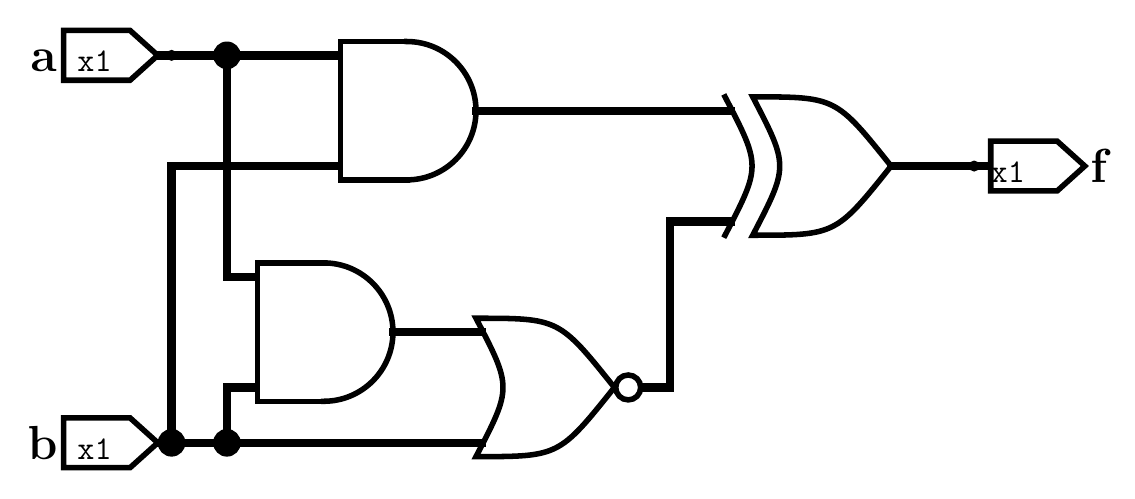
\begin{tikzpicture}[x=1pt,y=-1pt,line cap=rect]
\def\logisimfontA#1{\fontfamily{cmr}{#1}} % Replaced by logisim, original font was "SansSerif"
\def\logisimfontB#1{\fontfamily{cmtt}{#1}} % Replaced by logisim, original font was "Monospaced"
\definecolor{custcol_0_0_0}{RGB}{0, 0, 0}
\definecolor{custcol_ff_ff_ff}{RGB}{255, 255, 255}
\draw [line width=3.0pt, custcol_0_0_0 ]  (317.0,55.0) -- (347.0,55.0) ;
\draw [line width=3.0pt, custcol_0_0_0 ]  (117.0,55.0) -- (57.0,55.0) -- (57.0,155.0) -- (77.0,155.0) ;
\draw [line width=3.0pt, custcol_0_0_0 ]  (117.0,15.0) -- (77.0,15.0) -- (77.0,95.0) -- (87.0,95.0) ;
\fill [line width=3.0pt, custcol_0_0_0]  (57.0,155.0) ellipse (5.0 and 5.0 );
\fill [line width=3.0pt, custcol_0_0_0]  (77.0,15.0) ellipse (5.0 and 5.0 );
\fill [line width=3.0pt, custcol_0_0_0]  (77.0,155.0) ellipse (5.0 and 5.0 );
\draw [line width=3.0pt, custcol_0_0_0 ]  (52.0,155.0) -- (57.0,155.0) ;
\draw [line width=2.0pt, custcol_0_0_0 ]  (42.0,164.0) -- (52.0,155.0) -- (42.0,146.0) -- (18.0,146.0) -- (18.0,164.0) -- cycle;
\logisimfontB{\fontsize{12pt}{12pt}\selectfont\node[inner sep=0, outer sep=0, custcol_0_0_0, anchor=base west] at  (23.0,161.0)  {x1};}
\logisimfontA{\fontsize{16pt}{16pt}\fontseries{bx}\selectfont\node[inner sep=0, outer sep=0, custcol_0_0_0, anchor=base west] at  (5.0,161.0)  {b};}
\fill [line width=2.0pt, custcol_0_0_0]  (57.0,155.0) ellipse (2.0 and 2.0 );
\draw [line width=3.0pt, custcol_0_0_0 ]  (137.0,115.0) -- (167.0,115.0) -- (169.0,115.0) ;
\draw [line width=3.0pt, custcol_0_0_0 ]  (87.0,135.0) -- (77.0,135.0) -- (77.0,155.0) -- (167.0,155.0) -- (169.0,155.0) ;
\draw [line width=2.0pt, custcol_0_0_0 ]  (217.0,135.0) .. controls  (197.0,110.0)  ..  (167.0,110.0) .. controls  (180.0,135.0)  ..  (167.0,160.0) .. controls  (197.0,160.0)  ..  (217.0,135.0) -- cycle ;
\draw [line width=2.0pt, custcol_0_0_0]  (222.0,135.0) ellipse (4.5 and 4.5 );
\draw [line width=2.0pt, custcol_0_0_0] (112.0,140.0) arc (90.0:-90.0:25.0 and 25.0 );
\draw [line width=2.0pt, custcol_0_0_0 ]  (112.0,90.0) -- (88.0,90.0) -- (88.0,140.0) -- (112.0,140.0) ;
\draw [line width=3.0pt, custcol_0_0_0 ]  (52.0,15.0) -- (57.0,15.0) -- (77.0,15.0) ;
\draw [line width=2.0pt, custcol_0_0_0 ]  (42.0,24.0) -- (52.0,15.0) -- (42.0,6.0) -- (18.0,6.0) -- (18.0,24.0) -- cycle;
\logisimfontB{\fontsize{12pt}{12pt}\selectfont\node[inner sep=0, outer sep=0, custcol_0_0_0, anchor=base west] at  (23.0,21.0)  {x1};}
\logisimfontA{\fontsize{16pt}{16pt}\fontseries{bx}\selectfont\node[inner sep=0, outer sep=0, custcol_0_0_0, anchor=base west] at  (6.0,21.0)  {a};}
\fill [line width=2.0pt, custcol_0_0_0]  (57.0,15.0) ellipse (2.0 and 2.0 );
\draw [line width=3.0pt, custcol_0_0_0 ]  (167.0,35.0) -- (257.0,35.0) -- (259.0,35.0) ;
\draw [line width=3.0pt, custcol_0_0_0 ]  (227.0,135.0) -- (237.0,135.0) -- (237.0,75.0) -- (257.0,75.0) -- (259.0,75.0) ;
\draw [line width=2.0pt, custcol_0_0_0 ]  (317.0,55.0) .. controls  (297.0,30.0)  ..  (267.0,30.0) .. controls  (280.0,55.0)  ..  (267.0,80.0) .. controls  (297.0,80.0)  ..  (317.0,55.0) -- cycle ;
\draw [line width=2.0pt, custcol_0_0_0 ]  (257.0,30.0) .. controls  (270.0,55.0)  ..  (257.0,80.0) ;
\draw [line width=3.0pt, custcol_0_0_0 ]  (351.0,55.0) -- (348.0,55.0) ;
\draw [line width=2.0pt, custcol_0_0_0 ]  (377.0,46.0) -- (387.0,55.0) -- (377.0,64.0) -- (353.0,64.0) -- (353.0,46.0) -- cycle;
\logisimfontB{\fontsize{12pt}{12pt}\selectfont\node[inner sep=0, outer sep=0, custcol_0_0_0, anchor=base west] at  (353.0,61.0)  {x1};}
\logisimfontA{\fontsize{16pt}{16pt}\fontseries{bx}\selectfont\node[inner sep=0, outer sep=0, custcol_0_0_0, anchor=base west] at  (389.0,61.0)  {f};}
\fill [line width=2.0pt, custcol_0_0_0]  (347.0,55.0) ellipse (2.0 and 2.0 );
\draw [line width=2.0pt, custcol_0_0_0] (142.0,60.0) arc (90.0:-90.0:25.0 and 25.0 );
\draw [line width=2.0pt, custcol_0_0_0 ]  (142.0,10.0) -- (118.0,10.0) -- (118.0,60.0) -- (142.0,60.0) ;
\end{tikzpicture}
}

		\caption{Passarinho... Resolve esse... Qual é a expressão desse?\footnote[frame]{\textit{referência de velho}}}
		\label{fig:05exe}
	\end{figure}
\end{frame}